\subsection*{Samples}

\subsection*{Experimental setup}
\begin{figure}[ht]
	\centering
	\includegraphics{figures/experimentalSetup.png}
	\caption{Diagram of the photoluminescence spectroscopy setup.}
	\label{fig:experimentalSetup}
\end{figure}

As an excitation source a blue laser diode with a central wavelength of 402 ± 3 nm. A band-pass filter was placed after the diode to narrow down the excitation to 405 ± 10 nm. To reflect the excitation beam on to the sample and to transmit the emitted light from the sample a 425 nm dichroic long-pass filter. An achromatic lens was placed between the sample and dichroic mirror, to focus the excitation beam on the sample which simultaneously also collimates the emission from the sample. Since the dichroic mirror wasn’t sufficient in blocking the excitation light, an additional 420 nm long-pass filter after dichroic mirror was used to further block the excitation beam. A fiber coupling lens was placed after the filter to couple the PL emission in to the optical fiber. The optical fiber was then attached to an optical spectrometer (LR2 spectrometer from Lasertack, GmbH). The spectrometer covers a wavelength range from 200–1100 nm with <1 nm resolution. The integration time of spectrometer was set to a particular value. A microcontroller was used to regulate the laser power until sufficient PL signal was detected. If no signal was obtained at maximum out power of the laser the integration time of the spectrometer was increased. To compensate for non-uniformity in measurements due to undesired photobleaching at high powers, the spectrometer was turned on 500 ms after the laser using a microcontroller. 
Samples were placed on a two axis mototised stage to perform raster scanning. Before acquiring the PL spectra from samples, to eliminate any artifacts in the PL spectra a background spectrum was recorded by blocking the laser light, which was then subtracted from the PL spectra. 
